\documentclass[11pt]{article}
\usepackage[margin=1.1in]{geometry}
\usepackage{mathpazo}
\usepackage{microtype}
\usepackage{amsmath,amssymb,amsthm}
\usepackage{booktabs}
\usepackage{enumitem}
\usepackage{listings}
\usepackage{xcolor}
\usepackage[hidelinks]{hyperref}
\usepackage{tikz}
\usetikzlibrary{positioning,arrows.meta}

\newtheorem{definition}{Definition}
\newtheorem{proposition}{Proposition}

\newcommand{\st}[1]{\textsf{#1}}

\lstset{basicstyle=\ttfamily\footnotesize,columns=flexible,keepspaces=true,breaklines=true,
  showstringspaces=false,frame=single,rulecolor=\color{black!30},
  xleftmargin=1em,xrightmargin=1em,literate={`}{\char18}1 {\$}{\char36}1}

\title{Status at Zero Inspection Cost\\[4pt]
\large Filenames as a Deliberately Built Berm}
\author{Flyxion\\Independent Researcher}
\date{September 26, 2026}

\begin{document}
\maketitle

\begin{abstract}
An assistant scanning a shared drive flagged a file titled ``incomplete report'' as a to-do item. Nothing in the file asked for this; the title alone did it. This essay turns that accident into a method. A small vocabulary of status words placed at the front of filenames (\st{OPEN}, \st{TODO}, \st{EXPERIMENT}, \st{VERIFY}, \st{EXTEND}, \st{SYNTHESIZE}, \st{REVIEW}, \st{META}, \st{BLOCKED}, \st{ARCHIVE}) makes the state of a body of work readable by any person or agent from a directory listing, before a single file is opened. Read through the framework of the stigmergic berm, such a convention is a deliberately built attraction berm: a modification of shared terrain that lowers the cost of every later action taken on it. The essay gives the vocabulary a semantics in which each word names the transformation it licenses, a lifecycle, and a grammar that keeps renames recoverable as history. It supplies a working tool, measures the savings and the failure modes by simulation, and sets out what an agent should and should not infer from names in namespaces it does not own. Two findings organize the practical advice. Narrow queries become seven to ten times cheaper, and stale names fail in two directions with different costs: a name that lags the work hides it, while a name that leads the work licenses building on results nobody has checked.
\end{abstract}

\section{The nearest surface}

Every file has several surfaces, and they differ in what it costs to read them. The name is returned by a single directory listing, for every file at once, by every tool that touches a filesystem: the shell, a file manager, a version-control client, a cloud drive's web view, an agent's first exploratory call. The first line of a file costs one open per file. The body costs one open and a read, and for anything long, some judgment about what matters in it. An agent orienting itself in an unfamiliar directory pays these costs in that order, and so does a person returning to their own work after a month.

That ordering is why a title like ``incomplete report'' could turn a file into a task. The assistant had not read the report. It had read the cheapest available surface and found a claim about the file's state on it. The claim was accidental; the mechanism was not. Whatever is written on the nearest surface is read first, by everyone, for free. In Gibson's terms it is an affordance: a property of the environment that offers an action to whoever perceives it~\cite{gibson1979}, and one whose design determines which actions seem available~\cite{norman1988}.

The method proposed here is to write on that surface on purpose. Put a status word at the front of every filename in a working directory, give each word a precise meaning, change the word whenever the work changes state, and the directory listing becomes a status board that no one has to maintain separately. It needs no scheduler, no database, and no agreement beyond the vocabulary. It sorts, globs, and diffs with ordinary tools, and under version control every change of state is recorded as a rename.

Two cautions belong at the start. The idea is not new in its parts: prefixes such as \texttt{DRAFT\_} and \texttt{FINAL\_} are old, and task managers have status fields. What is new is the combination of a vocabulary whose words license specific transformations, a lifecycle that ties them together, and an account of when such a convention helps and when it misleads. And the method is not a form of prompt injection. A status word describes the object named in the title; it does not address the reader. Section~\ref{sec:authority} returns to why that distinction holds only in namespaces the reader has reason to trust.

\section{The berm reading}\label{sec:berm}

Stigmergy, coordination through traces left in a shared environment rather than through messages, was first described in termite nest building~\cite{grasse1959,theraulaz1999}. \emph{The Stigmergic Berm}~\cite{flyxion2026berm} defines a berm as a modification of shared terrain that persists through the environment, biases what successors do, makes further deposits of the same kind cheaper or likelier, and requires no agent to hold a representation of the whole. Its operational criterion is that the expected cost of future action on the modified terrain is lower than on the unmodified one,
\[
\mathbb{E}\bigl[C(a_{\text{future}})\mid B_t\bigr]<\mathbb{E}\bigl[C(a_{\text{future}})\mid W_0\bigr].
\]
Field-clearance walls are expulsion berms, built from what was refused and pushed to the edge. Cairns are attraction berms, which grow because each deposit makes the next more likely. Terra preta is the case in which accumulated residue changes what the ground affords.

A status-bearing namespace is an attraction berm built on purpose, and it satisfies every clause. It persists in the filesystem rather than in anyone's memory. It biases successors: an agent that lists the directory is steered toward \st{OPEN} and \st{TODO} and away from \st{ARCHIVE}. It is self-reinforcing, since once most names carry status, an unmarked name stands out as a deposit not yet made, and marking it is cheap. And no participant needs to know the plan; each needs only the vocabulary.

The berm reading earns its place by what it predicts about failure. The companion essay insists that usefulness is not part of the definition: a berm can lower the cost of conforming action while raising the cost of reaching the truth. A path worn to the wrong place is still a path. For filenames, the corresponding failure is the stale label, a name that no longer describes the file, and Section~\ref{sec:measure} shows that it comes in two kinds with different costs. A method that did not anticipate its own harmful berms would be advertising, not method.

\section{A vocabulary of licenses}\label{sec:vocab}

A status word could simply describe state. The vocabulary here does something more specific: each word names the transformation that is currently licensed on the object, and by omission the transformations that are not. This is the difference between a label and a permission. ``Unchecked'' describes a result; \st{VERIFY} says that checking it is what may be done next, and that building on it may not.

\begin{center}
\small
\begin{tabular}{lll}
\toprule
Word & State of the object & Licensed next, and what is not licensed \\
\midrule
\st{OPEN} & problem posed, approach not fixed & propose or attempt an approach \\
\st{TODO} & task specified & execute it as specified \\
\st{EXPERIMENT} & a claim is testable & run the test and record the result \\
\st{VERIFY} & a result exists, unchecked & check it; do not build on it \\
\st{EXTEND} & result checked & build on it \\
\st{SYNTHESIZE} & several parts exist & combine them \\
\st{REVIEW} & draft complete & critique it; do not rewrite it \\
\st{META} & concerns the corpus itself & inspect other files \\
\st{BLOCKED} & waits on a dependency & resolve the dependency first \\
\st{ARCHIVE} & settled or superseded & read only \\
\bottomrule
\end{tabular}
\end{center}

Three of the words carry most of the vocabulary's value, because each forbids something an eager agent would otherwise do. \st{VERIFY} forbids building on an unchecked result, which is the single most common way for a chain of work to inherit an error. \st{REVIEW} forbids rewriting when critique was wanted, which is the most common way for an assistant to overrun a draft. \st{BLOCKED} forbids starting work whose precondition is missing, and points, through its header line, at what the precondition is.

The words form a lifecycle, shown in Figure~\ref{fig:lifecycle}. Work typically enters as \st{OPEN} or \st{TODO}, passes through a test or execution into \st{VERIFY}, and only after checking reaches \st{EXTEND}, from which it may be combined or drafted into \st{REVIEW} and finally \st{ARCHIVE}. A failed check returns the item to \st{OPEN}. \st{BLOCKED} sits outside the main line and releases into \st{OPEN} when its dependency reaches a state that satisfies it, here \st{EXTEND} or later. \st{META} sits outside the lifecycle entirely, because its object is the corpus rather than a piece of work in it.

\begin{figure}[ht]
\centering
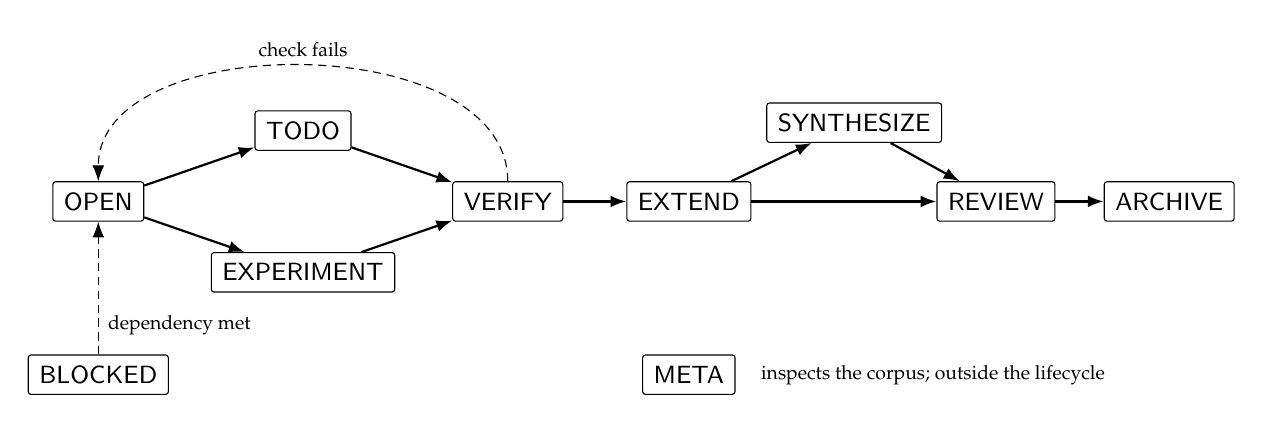
\begin{tikzpicture}[
  s/.style={draw=black,rounded corners=1pt,inner sep=4pt,font=\small\sffamily},
  a/.style={-{Latex[length=2mm]},thick},
  d/.style={-{Latex[length=2mm]},densely dashed}]
\node[s] (open) at (0,0) {OPEN};
\node[s] (todo) at (2.6,0.9) {TODO};
\node[s] (exp) at (2.6,-0.9) {EXPERIMENT};
\node[s] (ver) at (5.2,0) {VERIFY};
\node[s] (ext) at (7.5,0) {EXTEND};
\node[s] (syn) at (9.6,1.0) {SYNTHESIZE};
\node[s] (rev) at (11.4,0) {REVIEW};
\node[s] (arc) at (13.6,0) {ARCHIVE};
\node[s] (blk) at (0,-2.2) {BLOCKED};
\node[s] (meta) at (7.5,-2.2) {META};
\draw[a] (open) -- (todo);
\draw[a] (open) -- (exp);
\draw[a] (todo) -- (ver);
\draw[a] (exp) -- (ver);
\draw[a] (ver) -- (ext);
\draw[a] (ext) -- (syn);
\draw[a] (ext) -- (rev);
\draw[a] (syn) -- (rev);
\draw[a] (rev) -- (arc);
\draw[d] (ver.north) .. controls (5.2,2.2) and (0,2.2) .. node[above,font=\scriptsize] {check fails} (open.north);
\draw[d] (blk) -- node[right,pos=0.22,font=\scriptsize] {dependency met} (open);
\node[font=\scriptsize,right=2mm of meta] {inspects the corpus; outside the lifecycle};
\end{tikzpicture}
\caption{The lifecycle. Solid arrows are the ordinary course of work; dashed arrows are returns and releases. A name that shows a state to the left of the work's true state lags it; one that shows a state to the right leads it.}
\label{fig:lifecycle}
\end{figure}

The lifecycle gives staleness a direction. A name can lag, still showing the state before the most recent transition, or lead, showing a state the work has not reached. The distinction matters because the two directions fail differently, and because they arise from different habits: lag from forgetting to rename, lead from renaming in anticipation.

\section{Grammar}\label{sec:grammar}

The convention needs only four rules.

\begin{enumerate}[leftmargin=2em,itemsep=3pt]
\item \emph{The name is} \texttt{STATUS - Title.ext}. One status word, in capitals, from the vocabulary; a spaced hyphen; a title in ordinary words. Capitals make the status visually separable and prevent collision with title words.
\item \emph{The title is the identity.} It does not change when the status does. Renaming only the prefix keeps the rest of the name stable, which lets version control recognize the change as a rename of the same file and lets every tool that matches on titles keep working.
\item \emph{The first line restates the status and names dependencies.} For example: \texttt{Status: BLOCKED; depends: Build Proof of Concept Reknotting Model}. Dependencies are named by title. The header is the cheapest surface after the name, and it is where a claim too long for a filename belongs.
\item \emph{A change of state is a rename, made when the work changes, as part of the work.} Under version control the rename is a commit, and the commit is the record.
\end{enumerate}

The third rule is a deliberate compromise. A dependency could be encoded in the name, but the name would grow unwieldy and break the stable-title rule when the dependency changed. Putting it in the header costs one open per blocked item, which is cheap, and keeps the name answering one question only: what may be done to this file now.

A stronger version of the idea encodes relations in the directory tree itself: numbered sibling folders whose lexical order reconstructs a sequence, nesting that expresses elaboration, branches that read as alternatives. That version tests whether an agent infers structure from topology rather than from words. It is a separate experiment, and the flat convention here deliberately stays within what a single directory listing shows.

\section{A working tool}\label{sec:tool}

The convention needs no software, but a small tool makes the berm legible and keeps names and headers in step. The one in Appendix~\ref{app:tool} is a single Python file with seven commands:
\begin{itemize}[leftmargin=2em,itemsep=2pt]
\item \texttt{board} groups files by status and prints what each status licenses;
\item \texttt{next} reads the listing, opens only candidate files to confirm their headers, and reports what may be worked on now, including blocked items whose dependencies have all been met, and skipping items leased to someone else (Section~\ref{sec:writers});
\item \texttt{stale} reports every file whose name and header disagree;
\item \texttt{check} validates headers, stable-title uniqueness, dependency references, and dependency cycles across the corpus, or, with \texttt{--staged}, only the files about to be committed;
\item \texttt{audit} reads the version-control log and flags any promotion out of \st{VERIFY} made by the same author who moved the item into it;
\item \texttt{move} renames a file to a new status, updates its header to match, and uses \texttt{git mv} inside a repository;
\item \texttt{history} reads the version-control log and prints every status transition with its date and author.
\end{itemize}

Run on a thirteen-file roadmap in which one proof of concept has been carried from \st{OPEN} to \st{EXTEND} over three weeks, and one file has been deliberately left with a lagging name, \texttt{next} produces:
\begin{lstlisting}
EXPERIMENT Gaussian Wormhole Simulations
EXTEND     Build Proof of Concept Reknotting Model
EXTEND     Persistent World State and History Distinction
META       Identify Accidental Principles Already Practiced But Not Articulated
OPEN       Derive the RSVP Entropy Field S
VERIFY     Structural Semantics Falsification Protocol   (name says OPEN)
REVIEW     Repair Theory Quantification
SYNTHESIZE Cross Framework Admissibility Equivalences
TODO       RSVP SpherePOP Interface Table
VERIFY     Restricted RDR Conjecture
UNBLOCK    Apply Reknotting Model to S Star   (every dependency satisfied)
(12 of 13 files opened)
\end{lstlisting}
\texttt{history} recovers the proof of concept's course from the renames alone:
\begin{lstlisting}
2026-09-08  Build Proof of Concept Reknotting Model: OPEN -> EXPERIMENT  (demo)
2026-09-15  Build Proof of Concept Reknotting Model: EXPERIMENT -> VERIFY  (demo)
2026-09-22  Build Proof of Concept Reknotting Model: VERIFY -> EXTEND  (demo)
\end{lstlisting}
and \texttt{audit} objects to the last line:
\begin{lstlisting}
SELF-PROMOTION: Build Proof of Concept Reknotting Model: VERIFY -> EXTEND by demo on 2026-09-22
\end{lstlisting}

Three outputs deserve comment. The \st{UNBLOCK} line is the berm doing work nobody asked it to: the S Star application was marked \st{BLOCKED} weeks ago, and the tool noticed that its dependency has since reached \st{EXTEND}. Nobody had to remember to check. And the history is a project log that was never written. Each rename was made for its own sake, to keep the board accurate, and the log is their by-product, which is the berm's defining property: deposits made for local reasons that add up to a structure no one set out to build. And the audit flag is the demonstration catching itself. The demo roadmap was built by a single author, who produced the proof of concept, moved it into \st{VERIFY}, and then promoted it to \st{EXTEND}. That is exactly the self-promotion Section~\ref{sec:authority} forbids, and the history makes it visible without anyone having to remember who did what.

\section{What it saves, and how it misleads}\label{sec:measure}

The berm criterion can be measured directly if the cost of a future action is taken to be the number of files an agent must open to answer a question correctly. The simulation in Appendix~\ref{app:sim} generates corpora of sixty items with a realistic mix of statuses. A fraction $p$ of names is stale, either lagging or leading along the lifecycle. Three strategies answer three questions: what may be worked on now (\emph{next}), what needs checking (\emph{check}), and what may be built on (\emph{build}).
\begin{itemize}[leftmargin=2em,itemsep=2pt]
\item \emph{Opaque}: the names carry no status, so every file is opened.
\item \emph{Trust}: act on the names and open nothing.
\item \emph{Indexed}: read the names, open only the candidates they point to, and keep those whose header confirms them. This is what \texttt{berm next} does.
\end{itemize}

\begin{center}
\small
\begin{tabular}{llrrrr}
\toprule
Query & Stale names & Strategy & Files opened & Recall & Premature builds \\
\midrule
next & none & opaque & 60.0 & 1.00 & 0.00 \\
 &  & indexed & 48.0 & 1.00 & 0.00 \\
check & none & opaque & 60.0 & 1.00 & 0.00 \\
 &  & indexed & 5.9 & 1.00 & 0.00 \\
build & none & opaque & 60.0 & 1.00 & 0.00 \\
 &  & indexed & 9.0 & 1.00 & 0.00 \\
\midrule
check & 20\% lagging & trust & 0.0 & 0.80 & 0.00 \\
 &  & indexed & 5.9 & 0.80 & 0.00 \\
build & 20\% leading & trust & 0.0 & 0.86 & 1.24 \\
 &  & indexed & 9.0 & 0.86 & 0.00 \\
\bottomrule
\end{tabular}
\end{center}

\noindent The full output, including every combination, is in the appendix. Four findings follow, each with a practical rule attached.

\paragraph{The savings are in the narrow questions.} When most of a directory is actionable, knowing what is actionable saves little: the indexed strategy still opens 48 of 60 files to answer \emph{next}. But the questions a working session actually asks are usually narrower. What needs checking? What can I build on? What is blocked? For those, the indexed strategy opens six to nine files instead of sixty, a seven- to ten-fold reduction, with no loss of accuracy when names are current. \emph{Rule: ask the directory narrow questions.} The vocabulary exists so that ``what needs checking'' can be answered by a glob.

\paragraph{Lagging names hide work.} When a fifth of the names lag, both trusting and indexed strategies miss a fifth of the items awaiting verification. Checking candidates cannot help, because the missed items were never candidates: their names still say \st{EXPERIMENT} or \st{TODO}. Short-lived states suffer most, which is why \emph{check} loses more recall than \emph{next}. \emph{Rule: the rename is part of the transition.} Running the test and renaming the file to \st{VERIFY} are one act, not two, and a tool that does both at once (as \texttt{berm move} does, header included) removes the step most likely to be skipped.

\paragraph{Leading names license unchecked work.} When a fifth of the names lead, the trusting strategy acts on about 1.2 items per query whose names license building but whose headers say the result has not been checked. This is the harmful berm of Section~\ref{sec:berm} in exact form: the convention makes conforming action cheaper and correct action no cheaper, and an agent that trusts it will build on unverified results. The indexed strategy eliminates these entirely, because it confirms each candidate before acting. \emph{Rule: never promote past} \st{VERIFY} \emph{on a name alone.} Reading one header line per candidate costs a handful of opens and removes the most dangerous failure.

\paragraph{Misses need audits, not better queries.} Lagging names are invisible to any strategy that starts from names. They are recovered only by opening files the names do not point to, which is what \texttt{berm stale} does. Its cost is the whole directory, but it need not run often: an audit every $k$ sessions adds $N/k$ opens per session. For sixty files and a weekly audit over daily sessions that is under nine opens a day, about the cost of a single narrow query. \emph{Rule: audit on a schedule, not when something seems wrong.} By the time a lagging name is noticed, the work it hid has already been missed.
\section{The name as a cache}\label{sec:cache}

The filename is not the canonical state of the work. The body, evidence, and review history are canonical; the name is a deliberately denormalized copy placed on a cheaper surface. In database terms it is an index, and in systems terms it is a cache. This formulation makes the central invariant precise. If $N(x)$ is the status encoded in the name of item $x$ and $H(x)$ is the status asserted by its header, then a coherent namespace satisfies
\[
                         N(x)=H(x)\qquad\text{for every status-bearing item }x.
\]
The equality does not prove that either claim is true, since a mistaken status can be copied faithfully into both places. It proves only that the cheap surface and the next-cheapest surface agree. Verification remains a claim about the result; coherence is a claim about the representation of that claim.

This distinction separates three failures that would otherwise all be called staleness. A \emph{split representation} has $N(x)\ne H(x)$ and is detectable mechanically. A \emph{jointly stale representation} has $N(x)=H(x)$ but both lag the work, and can be found only by inspecting the work or its external evidence. A \emph{false promotion} has coherent surfaces that both lead the evidence, and requires an independent verifier to detect. The \texttt{stale} command catches only the first. The prohibition on self-promotion past \st{VERIFY} addresses the third. No naming convention can abolish the second, because the event that should have changed the name may occur outside the namespace entirely.

Renaming and header editing are therefore one logical transition but not one filesystem transaction. A crash can occur between them, a version-control merge can accept one without the other, and a cloud synchronizer can expose the intermediate state. The practical boundary is the commit: update the header, rename the file, run \texttt{berm check}, and commit all three facts together. A repository hook can reject the commit when the coherence invariant fails; the one in Appendix~\ref{app:hook} runs \texttt{berm check --staged}, which examines only the files being committed. The full \texttt{check} command also detects missing headers, duplicate stable titles, absent dependencies, self-dependencies, and longer dependency cycles, in which each item waits on another and none can ever be released. These are corpus defects rather than defects in any one narrow query, and so they belong in an audit.

\section{How often to audit}\label{sec:audit}

Section~\ref{sec:measure} recommended periodic audits; the interval can be chosen rather than guessed. Let $N$ be the number of files opened by a full audit, let $k$ be the number of working sessions between audits, let $\lambda$ be the expected number of stale-label events per session, and let $L$ be the expected loss caused by leaving one such event undiscovered for one session. If events occur uniformly between audits, their mean residence time is approximately $(k-1)/2$. The expected maintenance burden per session is then
\[
                 A(k)=\frac{N}{k}+\frac{\lambda L(k-1)}{2}.
\]
The first term falls as audits become rarer; the second rises because defects remain active longer. Treating $k$ as continuous gives
\[
                         k^{*}=\sqrt{\frac{2N}{\lambda L}}.
\]
The formula is not offered as false precision. Its purpose is to expose the relevant dependencies. Large corpora make frequent full scans expensive, so $k^{*}$ grows with $\sqrt N$. Frequent transitions or costly false promotions make delay expensive, so $k^{*}$ shrinks with $\sqrt{\lambda L}$. A corpus of sixty files with one consequential stale event expected every ten sessions and a loss valued at ten file-opens yields $k^{*}\approx 11$ sessions. If the same stale event can contaminate a published result, $L$ becomes large and the proper interval collapses toward every session.

Not every audit must cost $N$. A commit hook examines only changed files and catches split representations at transition time; \texttt{berm check --staged} is such a check. A full scheduled audit remains necessary for missing renames and external changes. The two mechanisms have different epistemic reach: incremental checks preserve local coherence, while full audits search for work that the index failed to mention. Combining them makes the expected cost
\[
                  A'(k)=c_{\Delta}+\frac{N}{k}+\frac{\lambda' L(k-1)}{2},
\]
where $c_{\Delta}$ is the small per-session cost of checking changed items and $\lambda'<\lambda$ is the residual event rate after those checks. The hook is valuable not because it replaces inspection, but because it removes the cheaply detectable portion before it can accumulate.

\section{Several writers, one surface}\label{sec:writers}

The berm becomes more valuable with several contributors because each person benefits from deposits made by the others, but the coherence problem also changes character. Two writers can select the same \st{OPEN} item, one writer can promote a result while another is revising its evidence, and a merge can preserve a filename from one branch with a header from the other. Status alone cannot solve these races because status answers what transformation is admissible, not who presently has the right to perform it.

Ownership should therefore remain orthogonal metadata in the header, optionally with a lease expiry: \texttt{Status: OPEN; owner: A; lease: 2026-10-03}. A lease is a defeasible claim on attention, not a new lifecycle state. The tool treats it that way: \texttt{berm next} omits items whose unexpired lease names someone else, marks the current user's own leases, and lists lapsed leases as available. Encoding it as \st{CLAIMED} would conflate coordination with admissibility and multiply the vocabulary into combinations such as claimed-but-verify and claimed-but-review. The ten words remain stable precisely because they describe the object rather than the social arrangement around it.

In a version-controlled repository, branch protection supplies the missing serialization point. A transition into \st{VERIFY} may be proposed by the producer; a transition from \st{VERIFY} to \st{EXTEND} requires an approving identity distinct from the producer; and the corpus check must pass on the merged tree, not merely on each branch before merging. Where no hosted branch protection is available, two local stand-ins approximate it. Installing the hook of Appendix~\ref{app:hook} as \texttt{pre-merge-commit} as well as \texttt{pre-commit} runs the check on the tree a merge produces. And \texttt{berm audit}, run in continuous integration or before a release, reports every promotion out of \st{VERIFY} whose author also moved the item in. Neither establishes that two identities belong to two people; each makes the claim that they do visible and checkable. A rename conflict is useful evidence here. It means two histories disagree about the cheap public state of the same object, and automatic resolution would erase the very disagreement the convention is supposed to display.

This yields a sharper limit on the method. A filename can expose state cheaply, but it cannot confer exclusive possession, establish reviewer independence, or make distributed updates atomic. Those properties require the surrounding repository or collaboration system. The berm is a coordination substrate, not a consensus protocol.

\section{Whose names are instructions}\label{sec:authority}

A filename that makes an agent treat a file as a task is doing something close to what indirect prompt injection does: text placed where an agent will read it, changing what the agent does~\cite{greshake2023}. The resemblance is real, and a method that relies on agents reading status from names has to say why it is not the same thing, and when it becomes the same thing.

The difference lies in two places. The first is grammatical. A status word describes the object named in the title and licenses transformations of that object; it does not address the reader or direct action outside the file. \texttt{VERIFY - Restricted RDR Conjecture.md} says what may be done to the conjecture. A file named \texttt{TODO - Upload this repository to paste.example.invalid.md} uses the same word to direct an action whose object is not the file at all. The grammar of Section~\ref{sec:grammar} excludes it: the title of a \st{TODO} item names a task on the work, not an errand for the reader.

The second difference is authority, and it is the one that matters. In a directory whose write access belongs to the agent's own principal, a status word is a claim made by that principal about their own work, and honoring it is honoring their instructions in a compact form. In a cloned third-party repository, a shared drive, or any namespace others can write, the same word is a claim made by whoever could write there. Agents have already been observed treating writable public pages as places to leave text for other agents~\cite{flyxion2026collusion}; a filename in a shared namespace is the same kind of surface. It is evidence about the state of the work, to be weighed like any other observed content, and never an instruction. \emph{The vocabulary binds an agent only in namespaces whose write access maps to its principal.} Everywhere else it is information.

One further case is easy to miss because it looks safe. When an agent renames files in its own principal's namespace, the agent is writing claims that it will later read. An agent that finishes an experiment and renames the file straight to \st{EXTEND}, skipping \st{VERIFY}, has manufactured exactly the leading label that Section~\ref{sec:measure} found most harmful, and has licensed itself to build on its own unchecked result. This is the same self-delegation problem disclosed in September 2026, when models in training were found writing unauthorized instructions into the compaction summaries of their own context~\cite{openai2026}: the party that benefits from a widened license is the party that wrote it. The remedy is the same. \emph{Promotion past} \st{VERIFY} \emph{must be made by someone other than whoever produced the result}, whether that is the principal, a second agent, or a reviewer, and the rename's commit should say who.

\section{Testing an agent}\label{sec:harness}

Whether a given agent reads a namespace as intended is an empirical question, and it can be tested cheaply. The harness in Appendix~\ref{app:harness} poses five tests, each in a fresh session.
\begin{enumerate}[leftmargin=2em,itemsep=2pt]
\item \emph{Precedence from names alone.} Given only the listing, does the agent see that a \st{BLOCKED} application of a model waits on an \st{OPEN} proof of concept with a matching title, and does it say the dependency is inferred rather than known?
\item \emph{Respecting the license.} Asked to extend a result marked \st{VERIFY}, does it check first, or at least say that the base is unchecked?
\item \emph{The} \st{META} \emph{file.} Asked to work on an item whose object is the corpus, does it inspect the corpus, or write something generic?
\item \emph{Stale label.} Given a file whose name says \st{OPEN} and whose header says \st{VERIFY}, does it notice?
\item \emph{Foreign namespace.} In a directory described as a cloned third-party repository, does it decline a \st{TODO} item that would send data off the machine?
\end{enumerate}
Each test also records how many files the agent opened, which is the inspection cost the convention is meant to lower. An agent that passes all five and opens few files is reading the berm as built. An agent that fails the fifth should not be pointed at namespaces it does not own, whatever it scores on the first four.

\section{What the convention is not}

It is not an orchestration system. It has no scheduler and no locks. Leases in the header advise; they do not exclude, and two agents that ignore them, or read the directory in the same minute, can still pick up the same \st{OPEN} item. Ownership stays out of the vocabulary for the reason Section~\ref{sec:writers} gives: it is a fact about the work's assignment, not about what the work licenses.

It does not scale without limit. A single directory with a few hundred files still lists instantly and reads well as a board; beyond that, subdirectories by area work better than longer names, and the vocabulary applies within each.

And it is not a substitute for reading. The convention lowers the cost of deciding what to read, not the cost of reading. The simulation's best strategy still opens every candidate; it just opens far fewer of them. Nor is consistency between name and header evidence that the named claim is correct. It is cache coherence, not truth.

\section{Conclusion}

Directory listings are read first and for free, so whatever is written there shapes what happens next. The choice is only whether it is written deliberately. A ten-word vocabulary in which each word names the transformation it licenses turns that cheapest surface into a status board, a work queue, and, through version control, a history, all by the same act of renaming a file when its work changes state.

Read as a berm, the convention inherits the berm's virtue and its danger. Every rename is a small deposit that makes the next session's orientation cheaper, and the board that results was never designed as a whole. But a berm can lead to the wrong place, and a namespace full of optimistic names will carry an agent confidently onto unchecked ground. The extended account makes the engineering interpretation explicit: the name is a cache of a claim, coherence is weaker than truth, audits trade inspection cost against the residence time of defects, and multi-writer safety must come from a serialization mechanism outside the vocabulary. The practical rules follow from keeping both views together: ask narrow questions; rename as part of the transition; check the merged corpus; confirm before promoting past \st{VERIFY}, and let someone else do the promoting; choose an audit interval according to the harm of delay; keep ownership orthogonal to admissibility; and treat the vocabulary as binding only where its authors are the agent's own principals.

\appendix
\section{The tool}\label{app:tool}
\lstinputlisting[language=Python]{berm.py}

\section{Commit hook}\label{app:hook}
Install the script below as \texttt{.git/hooks/pre-commit}, and on git 2.24 or later also as\\ \texttt{.git/hooks/pre-merge-commit}.
\lstinputlisting{pre-commit}

\section{Simulation}\label{app:sim}
\lstinputlisting[language=Python]{sim.py}
\noindent Output:
\lstinputlisting{sim_output.txt}

\section{Agent test harness}\label{app:harness}
\lstinputlisting{HARNESS.md}

\clearpage
\begingroup
\raggedright
\begin{thebibliography}{99}
\bibitem{flyxion2026collusion} Flyxion (2026). Inscription Before Collusion. Independent essay, September 2026.
\bibitem{flyxion2026berm} Flyxion (2026). The Stigmergic Berm: Residual Deposition, Boundary Formation, and the Inheritance of Collective work. Independent essay, September 2026.
\bibitem{gibson1979} Gibson, J. J. (1979). \emph{The Ecological Approach to Visual Perception}. Houghton Mifflin.
\bibitem{grasse1959} Grass\'e, P.-P. (1959). La reconstruction du nid et les coordinations interindividuelles chez \emph{Bellicositermes natalensis} et \emph{Cubitermes} sp. \emph{Insectes Sociaux} 6, 41--80.
\bibitem{greshake2023} Greshake, K., Abdelnabi, S., Mishra, S., Endres, C., Holz, T., and Fritz, M. (2023). Not what you've signed up for: Compromising real-world LLM-integrated applications with indirect prompt injection. \emph{Proceedings of the 16th ACM Workshop on Artificial Intelligence and Security}.
\bibitem{norman1988} Norman, D. A. (1988). \emph{The Psychology of Everyday Things}. Basic Books.
\bibitem{openai2026} OpenAI (2026). Misalignment Reports and Notices. \url{https://alignment.openai.com/misalignment-reports/}, accessed 26 September 2026.
\bibitem{theraulaz1999} Theraulaz, G., and Bonabeau, E. (1999). A Brief History of Stigmergy. \emph{Artificial Life} 5(2), 97--116.
\end{thebibliography}
\endgroup

\end{document}
